\usetikzlibrary{arrows}
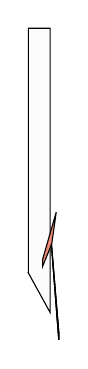
\begin{tikzpicture}
\definecolor{color1}{HTML}{FDFCFC}
\draw[fill=color1] (-0.0008368199384615384, 0.5030218444444444)-- (0.0008368200615384616, 0.5030218444444444)-- (0.0008368200615384616, 1.802533711111111)-- (0.0008368200615384616, 3.6080893333333335)-- (0.13929835692307693, 3.6080893333333335)-- (0.27775989538461543, 3.6080893333333335)-- (0.27775989538461543, 1.802533711111111)-- (0.27775989538461543, -0.0030218497777777776)-- cycle;
\definecolor{color2}{HTML}{F1A799}
\draw[fill=color2] (0.29024010461538463, 0.8674726888888888)-- cycle;
\definecolor{color3}{HTML}{ED8B75}
\draw[fill=color3] (0.29762472, 0.8682164666666666)-- (0.1815472, 0.582833022222222)-- (0.1815472, 0.6717219111111109)-- (0.3548924984615386, 1.2728191111111111)-- cycle;
\definecolor{color4}{HTML}{9D9EA0}
\draw[fill=color4] (0.2933170276923077, 0.8651442)-- cycle;
\definecolor{color5}{HTML}{E96856}
\draw[fill=color5] (0.2933170276923077, 0.8651442)-- cycle;
\definecolor{color6}{HTML}{7D7E80}
\draw[fill=color6] (0.29362472, 0.8628381333333333)-- (0.38782129230769224, -0.2672883111111114)-- (0.38782129230769224, -0.3506216444444447)-- cycle;
\definecolor{color7}{HTML}{636465}
\draw[fill=color7] (0.29362472, 0.8628381333333333)-- (0.38782129230769224, -0.2672883111111114)-- (0.38782129230769224, -0.3506216444444447)-- cycle;
\definecolor{color8}{HTML}{E22317}
\draw[fill=color8] (0.29362472, 0.8628381333333333)-- (0.38782129230769224, -0.2672883111111114)-- (0.38782129230769224, -0.3506216444444447)-- cycle;
\end{tikzpicture}
